\documentclass[12pt,a4paper,austrian]{article}
\usepackage{graphicx}
\usepackage[austrian, english]{babel}
\usepackage[utf8]{inputenc}
\usepackage{listings}
\usepackage{multirow}
\usepackage{epstopdf}
\usepackage{amsmath}
\usepackage{amssymb}
\usepackage{hyperref} % fuer Mengen \N, Q, C, R
\usepackage{minted} % fuer Code Listings mit Syntax Highlighting
\graphicspath{{./fig/}}


%% Satzspiegel
\setlength{\hoffset}{-1in} \setlength{\textwidth}{18cm}
\setlength{\oddsidemargin}{1.5cm}
\setlength{\evensidemargin}{1.5cm}
\setlength{\marginparsep}{0.7em}
\setlength{\marginparwidth}{0.5cm}

\setlength{\voffset}{-1.9in}
\setlength{\headheight}{12pt}
\setlength{\topmargin}{2.6cm}
\addtolength{\topmargin}{-\headheight}
\setlength{\headsep}{3.5cm}
\addtolength{\headsep}{-\topmargin}
\addtolength{\headsep}{-\headheight}
\setlength{\textheight}{27cm}

%% How should floats be treated?
\setlength{\floatsep}{12 pt plus 0 pt minus 8 pt}
\setlength{\textfloatsep}{12 pt plus 0pt minus 8 pt}
\setlength{\intextsep}{12 pt plus 0pt minus 8 pt}

\tolerance2000
\emergencystretch20pt

%% Text appearence
% English text
\newcommand{\eg}[1]%
{\selectlanguage{english}\textit{#1}\selectlanguage{austrian}}

\newcommand{\filename}[1]
{\begin{small}\texttt{#1}\end{small}}

\newcommand\IFT{\unitlength1mm\begin{picture}(10,2) \put (1,1)
{\circle{1.7}} \put(2,1){\line(1,0){5}} \put(8,1)
{\circle*{1.7}}\end{picture}}
\newcommand\FT{\unitlength1mm\begin{picture}(10,2) \put (1,1)
{\circle*{1.7}} \put(2,1){\line(1,0){5}} \put(8,1)
{\circle{1.7}}\end{picture}}

% A box for multiple choice problems
\newcommand{\choicebox}{\fbox{\rule{0pt}{0.5ex}\rule{0.5ex}{0pt}}}

\newenvironment{wahrfalsch}%
{\bigskip\par\noindent\makebox[1cm][c]{richtig}\hspace{3mm}\makebox[1cm][c]{falsch}
    \begin{list}%
    {\makebox[1cm][c]{\choicebox}\hspace{3mm}\makebox[1cm][c]{\choicebox}}%
    {\setlength{\labelwidth}{2.31 cm}\setlength{\labelsep}{3mm}
    \setlength{\leftmargin}{2.61 cm}\setlength{\listparindent}{0pt}
    \setlength{\itemindent}{0pt}}%
    }
    {\end{list}}

\newcounter{theaufgabe}\setcounter{theaufgabe}{1}
\newenvironment{aufgabe}[1]%
{\bigskip\par\noindent\begin{nopagebreak}
                          \textsf{\textbf{\arabic{theaufgabe}.\thinspace Aufgabe}}\quad
                          \textsf{\textit{#1}}\\*[1ex]%
                          \stepcounter{theaufgabe}\hspace{2ex}
\end{nopagebreak}}
{\par\pagebreak[2]}

% Innerhalb der Aufgaben erfolgt die weitere Unterteilung mittels einer
% enumerate Umgebung, die allerdings a), b),... zaehlen soll.
\renewcommand{\labelenumi}{\alph{enumi})}
\renewcommand{\labelenumii}{\arabic{enumii})}

% A box to tick for everything which has to done
\newcommand{\abgabe}{\marginpar{$\Box$}}
% Margin paragraphs on the left side
\reversemarginpar

% Language for listings
%\lstset{language=Vhdl,
%  basicstyle=\small\tt,
% keywordstyle=\tt\bf,
% commentstyle=\sl}

% No indention
\setlength{\parindent}{0.0cm}
% Don't number sections
\setcounter{secnumdepth}{0}


%% Beginning of the text

\begin{document}
    \selectlanguage{austrian}
    \pagestyle{plain}


%===  This is the header section ============================================================
    \thispagestyle{empty}
    \noindent
    \begin{minipage}[b][4cm]{1.0\textwidth}
        \begin{center}
            \begin{bf}
                \begin{large}
                    Digital Signal Processing SS 2024 -- 5.~Assignment
                \end{large} \\
                \vspace{0.3cm}
                \begin{Large}
                    z-Transform, Digital Filters
                \end{Large} \\
                \vspace{0.3cm}
            \end{bf}
            \begin{large}
                Group 22\\
                Julian Feichtinger, K12015812\\
                Wolfram Laube, K08900915\\
            \end{large}
        \end{center}
    \end{minipage}

    \noindent \rule[0.8em]{\textwidth}{0.12mm}\\[-0.5em]
%=======================================================================================


    \begin{aufgabe}{Signal Distortion and Group Delay (20\%)}

        Generate three periods of the signal

        $$
        x[n]=\sum_{i=1}^{4} \frac{1}{2 i-1} \sin (2 \pi 0.005(2 i-1) n)
        $$

        and load (MATLAB command load) the provided mat file \texttt{Filter\_coefficients.mat}.
        This file contains the filter coefficients of an FIR filter (b1 and a1) and the filter coefficients of an IIR filter (b2 and a2).
        Both filters are designed to fulfil the same design criteria (filter specification).
        Filter with both the FIR and the IIR filter the signal $x[n]$ and observe the signal distortion.
        Show and discuss the results in your report.

        \hrule
        \section*{Signal Distortion and Group Delay}

\subsection*{Problem Statement}
Generate three periods of the signal:
\[ x[n]=\sum_{i=1}^{4} \frac{1}{2 i-1} \sin (2 \pi 0.005(2 i-1) n) \]
Load the provided filter coefficients from \texttt{Filter\_coefficients.mat} and filter the signal using both FIR and IIR filters. Observe the signal distortion and discuss the results.

\subsection*{Theoretical Background}
This exercise involves generating a composite signal formed by summing four sinusoidal components with specific frequencies and amplitudes. The signal \( x[n] \) is given by:
\[ x[n]=\sum_{i=1}^{4} \frac{1}{2 i-1} \sin (2 \pi 0.005(2 i-1) n) \]

Filtering this signal using two different types of filters (FIR and IIR) allows us to observe how each filter type affects the signal.

\subsection*{Mathematical Derivation}
The formula for each component of the signal can be derived as:
\[ \text{Component}_i = \frac{1}{2i-1} \sin(2 \pi 0.005 (2i-1) n) \]
The final signal \( x[n] \) is the sum of these four components.

Given the filter coefficients \( b1, a1 \) for the FIR filter and \( b2, a2 \) for the IIR filter, the filtering process can be described as:
\[ y_{\text{FIR}}[n] = \text{filter}(b1, a1, x[n]) \]
\[ y_{\text{IIR}}[n] = \text{filter}(b2, a2, x[n]) \]

\subsection*{Implementation and Results}
The generated signal and the filtered signals are obtained through Python code. The plots below illustrate the generated signal and the filtered signals using both FIR and IIR filters.

\begin{figure}[h]
    \centering
    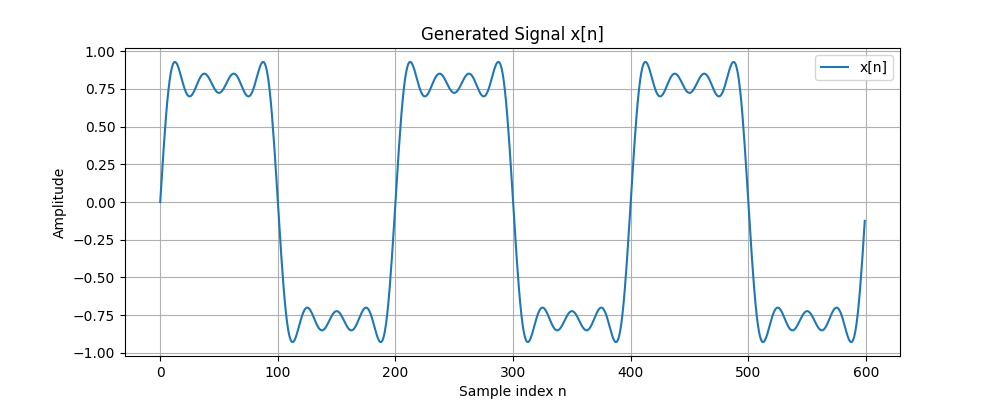
\includegraphics[width=0.8\textwidth]{fig/ex1_generated_signal.png}
    \caption{Generated Signal \( x[n] \)}
    \label{fig:ex1_generated_signal}
\end{figure}

\begin{figure}[h]
    \centering
    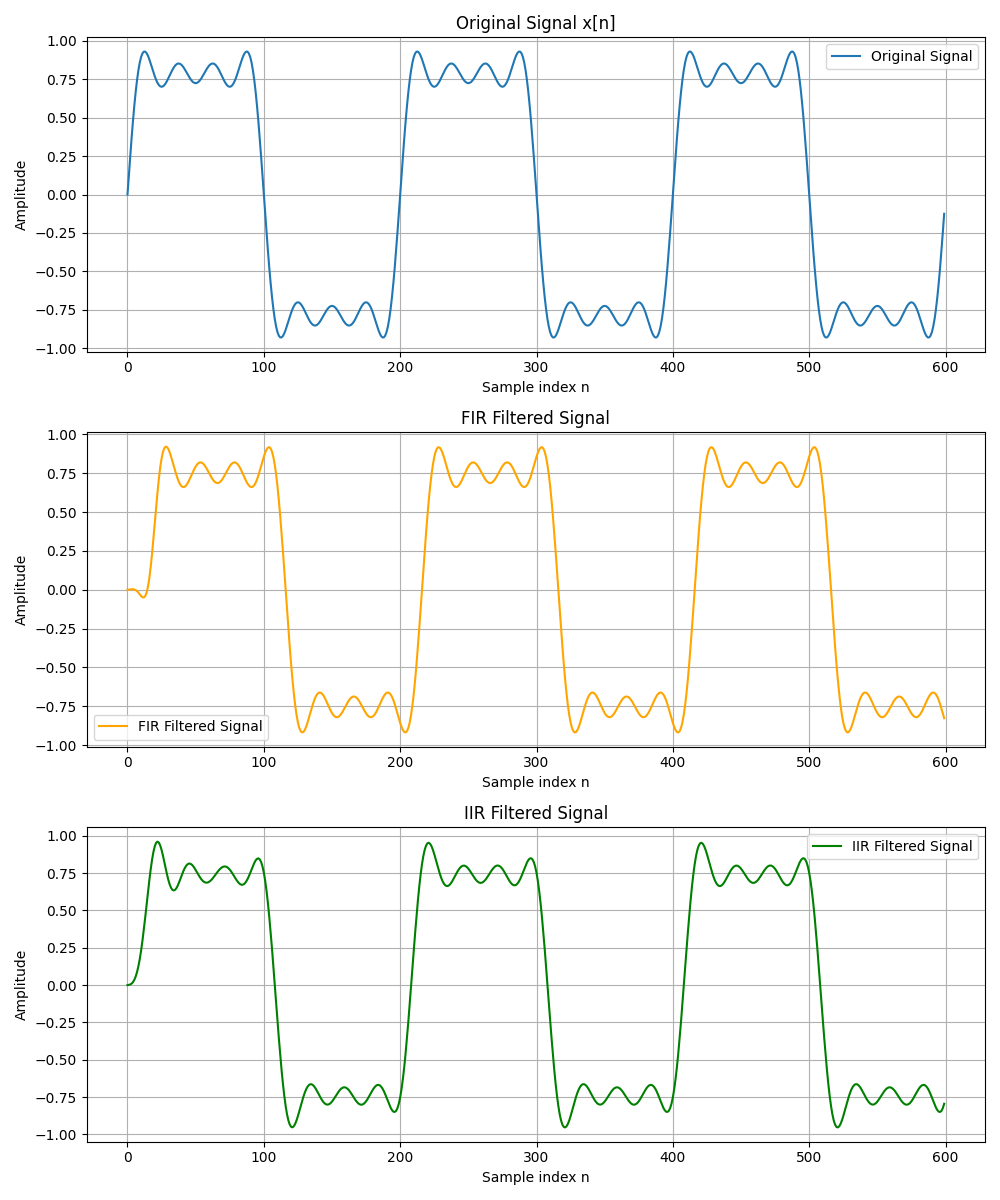
\includegraphics[width=0.8\textwidth]{fig/ex1_filtered_signals.png}
    \caption{Filtered Signals: FIR and IIR}
    \label{fig:ex1_filtered_signals}
\end{figure}

\subsection*{Conclusion}
The FIR and IIR filtered signals show how each filter type affects the original signal. FIR filters tend to introduce a uniform delay while preserving the waveform shape, whereas IIR filters can introduce phase distortions but achieve better magnitude response with a lower order.


    \end{aufgabe}

    \begin{aufgabe}{z-Transform (25\%)}

        Consider the difference equation of a recursive LTI system

        $$
        y[n]=x[n]-\frac{1}{15} y[n-1]+\frac{2}{5} y[n-2]
        $$

        \begin{enumerate}
            \item[(a)] Sketch the block diagram of the LTI system corresponding to the given difference equation.
            \item[(b)] Determine the filter type (FIR or IIR) and explain your choice in the report.
            \item[(c)] Compute the transfer function $H(z)=\frac{Y(z)}{X(z)}$.
            \item[(d)] Calculate the poles and zeros of $H(z)$ and include a sketch of the pole-zero map in your report.
            Also include the region of convergence (ROC) in the pole-zero map.
            \item[(e)] Is the system stable?
            Explain your answer.
        \end{enumerate}

        \hrule

        \begin{enumerate}
            %! Author = wolfram_e_laube
%! Date = 06.05.24

\item[(a)]
\subsection{Task (a): Real and Imaginary Parts of $X(f)$}

\subsubsection{Problem Statement}
Visualize the real and imaginary components of the frequency spectrum $X(f)$, given its magnitude $|X(f)|$ and phase $\phi_x(f)$, and discuss the implications of these components in signal processing.

\subsubsection{Mathematical Formulation}
Given:
\begin{itemize}
    \item \textbf{Magnitude $|X(f)|$:}
    \[
    |X(f)| =
    \begin{cases}
    A & \text{if } -5 \leq f < -1 \text{ or } 1 < f \leq 5 \\
    A(1 + f) & \text{if } -1 \leq f < 0 \\
    A(1 - f) & \text{if } 0 \leq f \leq 1 \\
    0 & \text{otherwise}
    \end{cases}
    \]

    \item \textbf{Phase $\phi_x(f)$:}
    \[
    \phi_x(f) =
    \begin{cases}
    \frac{\pi}{2} & \text{if } -5 \leq f < 0 \\
    -\frac{\pi}{2} & \text{if } 0 < f \leq 5 \\
    0 & \text{otherwise}
    \end{cases}
    \]
\end{itemize}

Using Euler's formula:
\[
X(f) = |X(f)| \cdot e^{i \phi_x(f)}
\]
\[
\text{Re}\{X(f)\} = |X(f)| \cos(\phi_x(f))
\]
\[
\text{Im}\{X(f)\} = |X(f)| \sin(\phi_x(f))
\]

\subsubsection{Discussion}
The real part $\text{Re}\{X(f)\}$ is zero for all $f$, reflecting the phase shifts of $\frac{\pi}{2}$ and $-\frac{\pi}{2}$. The imaginary part $\text{Im}\{X(f)\}$ shows variations with $f$, mirroring the magnitude adjustments and the sinusoidal phase behavior.

\begin{figure}[h]
    \centering
    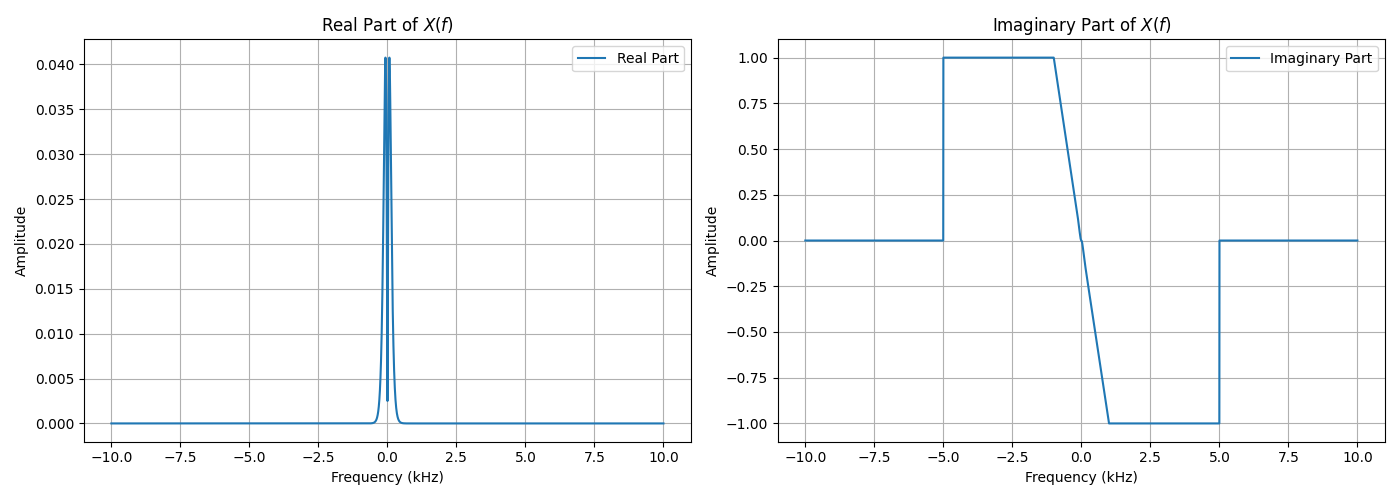
\includegraphics[width=0.49\textwidth]{fig/ex2_a_plot}
    \caption{Real and Imaginary Parts of $X(f)$}
    \label{fig:ex2_a_plot}
\end{figure}

            %! Author = wolfram_e_laube
%! Date = 06.05.24

\item[(b)]
\subsection{Task (b): Spectrum of $x[n]$}

\subsubsection{Problem Statement}
Analyze and visualize the spectrum of the discrete-time signal $x[n]$, obtained by sampling the continuous-time signal $x(t)$ at a frequency $f_s$, and elucidate the effects of sampling including aliasing.

\subsubsection{Mathematical Formulation}
\begin{itemize}
    \item \textbf{Sampling Frequency $f_s = 8$ kHz}
    \item \textbf{Baseband:} $[-f_s/2, f_s/2]$ or $[-4 \text{ kHz}, 4 \text{ kHz}]$
\end{itemize}

The spectrum $X(f)$ repeats every $f_s$, illustrating the aliasing effects:
\[
\text{Extended Frequency Range for Visualization: } [-3f_s, 3f_s]
\]
\[
\text{Repeated Spectrum: } \text{tile}( |X(f)|, 3)
\]

\subsubsection{Discussion}
The plot of $x[n]$ shows how the spectrum repeats every $f_s$ and highlights the baseband where the original spectrum lies within the Nyquist range. This visualization demonstrates the aliasing effect, where parts of the spectrum outside the baseband overlap with those inside it.

\begin{figure}[h]
    \centering
    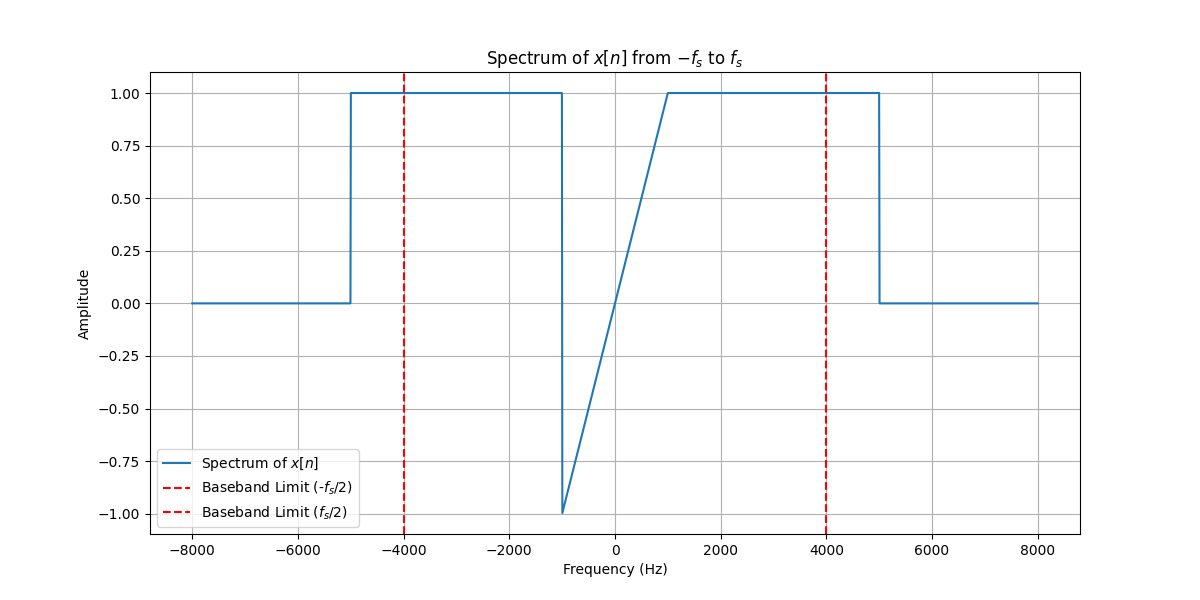
\includegraphics[width=0.49\textwidth]{fig/ex2_b_plot}
    \caption{Spectrum of \(x(t)\)}
    \label{fig:ex2_b_plot}
\end{figure}

            \item[(a)]
\section*{Task (a)}

\subsection*{Problem Statement}
% TODO insert problem statement here

\subsection*{Theoretical Background}
% TODO insert theoretical here

\subsection*{Mathematical Derivation}
% TODO insert mathematical derivation here

\subsection*{Python Implementation and Plot}
% TODO insert plot description here
The plot Figure~\ref{fig:ex1_a_plot} below illustrates these this

% TODO insert plot here
\begin{figure}[h]
    \centering
    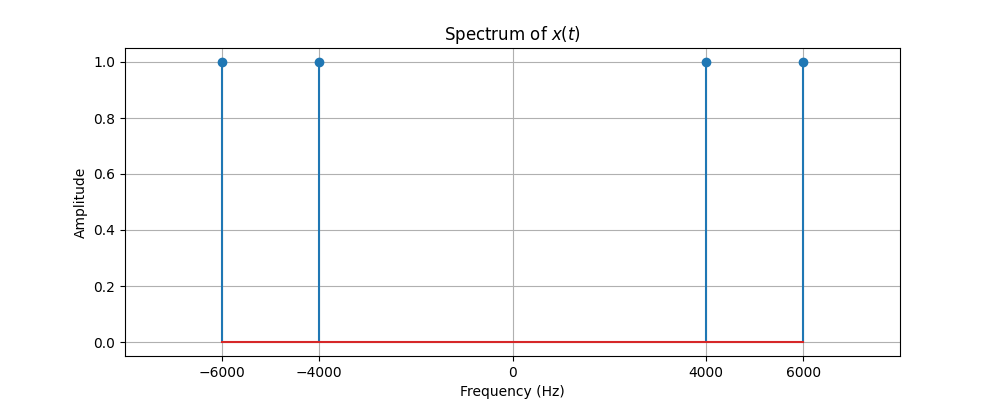
\includegraphics[width=0.8\textwidth]{fig/ex1_a_plot}
    \caption{Exercise 1 Task (a)}
    \label{fig:ex1_a_plot}
\end{figure}

\subsection*{Conclusion}
            \item[(a)]
\section*{Task (a)}

\subsection*{Problem Statement}
% TODO insert problem statement here

\subsection*{Theoretical Background}
% TODO insert theoretical here

\subsection*{Mathematical Derivation}
% TODO insert mathematical derivation here

\subsection*{Python Implementation and Plot}
% TODO insert plot description here
The plot Figure~\ref{fig:ex1_a_plot} below illustrates these this

% TODO insert plot here
\begin{figure}[h]
    \centering
    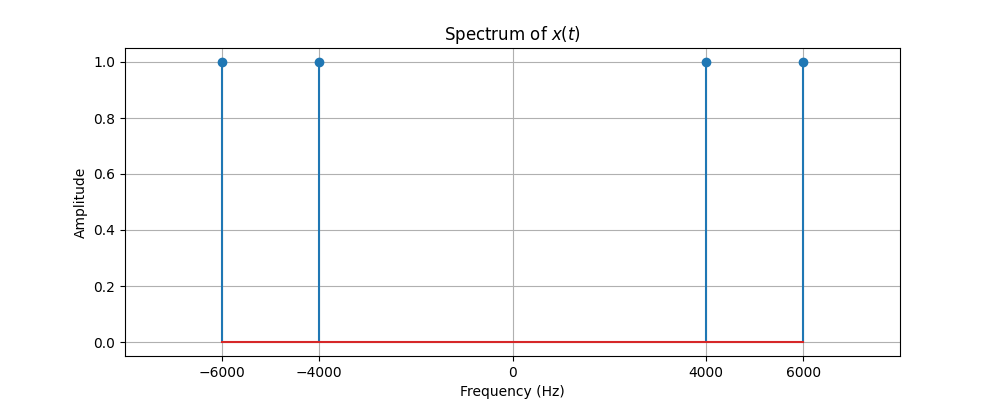
\includegraphics[width=0.8\textwidth]{fig/ex1_a_plot}
    \caption{Exercise 1 Task (a)}
    \label{fig:ex1_a_plot}
\end{figure}

\subsection*{Conclusion}
            \item[(a)]
\section*{Task (a)}

\subsection*{Problem Statement}
% TODO insert problem statement here

\subsection*{Theoretical Background}
% TODO insert theoretical here

\subsection*{Mathematical Derivation}
% TODO insert mathematical derivation here

\subsection*{Python Implementation and Plot}
% TODO insert plot description here
The plot Figure~\ref{fig:ex1_a_plot} below illustrates these this

% TODO insert plot here
\begin{figure}[h]
    \centering
    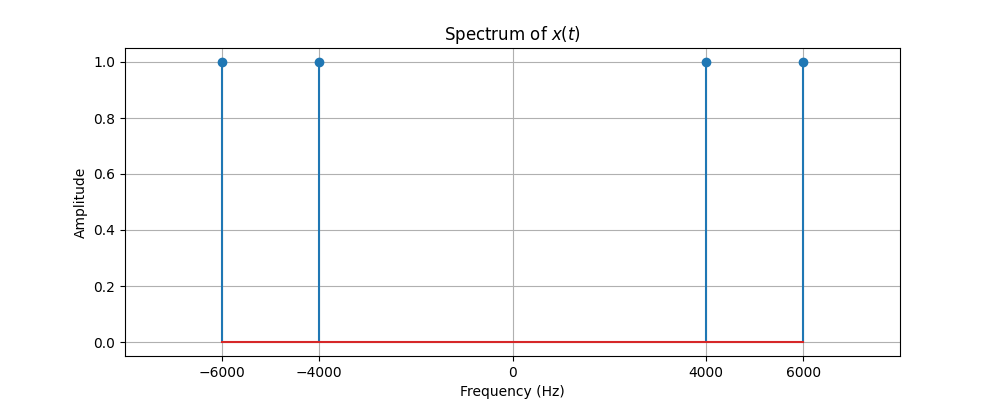
\includegraphics[width=0.8\textwidth]{fig/ex1_a_plot}
    \caption{Exercise 1 Task (a)}
    \label{fig:ex1_a_plot}
\end{figure}

\subsection*{Conclusion}
            \item[(f)]
\section{Derive the Difference Equation}

\subsection*{Problem Statement}
Given the poles and zeros, derive the difference equation from the transfer function \( H(z) \).

\subsection*{Theoretical Background}
The transfer function \( H(z) \) relates the input and output of a system in the z-domain. By expressing \( H(z) \) in terms of its polynomial coefficients, we can convert it back to the time-domain difference equation.

\subsection*{Mathematical Derivation}
The transfer function derived previously is:
\[ H(z) = \frac{z^2}{z^2 + \frac{1}{15} z - \frac{2}{5}} \]

We can express this as:
\[ H(z) = \frac{Y(z)}{X(z)} = \frac{z^2}{z^2 + \frac{1}{15} z - \frac{2}{5}} \]

This gives:
\[ Y(z) \left( z^2 + \frac{1}{15} z - \frac{2}{5} \right) = z^2 X(z) \]

In the time domain, this corresponds to the difference equation:
\[ y[n] + \frac{1}{15} y[n-1] - \frac{2}{5} y[n-2] = x[n] \]

Rearranging terms to isolate \( y[n] \):
\[ y[n] = x[n] - \frac{1}{15} y[n-1] + \frac{2}{5} y[n-2] \]

\subsection*{Conclusion}
The derived difference equation from the transfer function \( H(z) \) is:
\[ y[n] = x[n] - \frac{1}{15} y[n-1] + \frac{2}{5} y[n-2] \]
This confirms the given difference equation.

        \end{enumerate}

    \end{aufgabe}

    \begin{aufgabe}{Recursive Filter (25\%)}

        Let the poles and zeros of a recursive filter be given:
        \begin{enumerate}
            \item[-] Zeros: $N_{1}=-1, N_{2}=j, N_{3}=-j$
            \item[-] Poles: $P_{1}=0, P_{2}=0.75+j 0.25, P_{3}=0.75-j 0.25$
        \end{enumerate}

        \begin{enumerate}
            \item[(a)] Does this filter have real coefficients? Justify your answer.
            \item[(b)] Draw a sketch of the pole-zero map.
            \item[(c)] State the transfer function, first with polynomials of $z^{-i}, i=0,1,2,3, \ldots$, and afterwards with polynomials of $z^{+i}$.
            \item[(d)] Draw the block diagram of a direct-form-l implementation of the filter and specify the coefficient values in the block diagram.
            \item[(e)] Plot the magnitude and phase response of the filter in MATLAB.
            \item[(f)] Plot the impulse response of the filter for $0 \leq n \leq 50$ in MATLAB.
        \end{enumerate}

        \hrule

        \begin{enumerate}
            \item[(a)]
\section{Real Coefficients of the Filter}

\subsection*{Problem Statement}
Does this filter have real coefficients? Justify your answer.

Given:
\begin{itemize}
    \item Zeros: \( N_{1}=-1, N_{2}=j, N_{3}=-j \)
    \item Poles: \( P_{1}=0, P_{2}=0.75+j0.25, P_{3}=0.75-j0.25 \)
\end{itemize}

\subsection*{Theoretical Background}
A filter has real coefficients if the poles and zeros either occur in complex conjugate pairs or are real numbers. This ensures that the filter's impulse response is real.

\subsection*{Mathematical Derivation}
The given zeros are:
\begin{itemize}
    \item \( N_{1} = -1 \) (real)
    \item \( N_{2} = j \) (complex)
    \item \( N_{3} = -j \) (complex conjugate of \( j \))
\end{itemize}

The given poles are:
\begin{itemize}
    \item \( P_{1} = 0 \) (real)
    \item \( P_{2} = 0.75 + j0.25 \) (complex)
    \item \( P_{3} = 0.75 - j0.25 \) (complex conjugate of \( 0.75 + j0.25 \))
\end{itemize}

Since the zeros and poles either occur in complex conjugate pairs or are real numbers, the filter has real coefficients.

\subsection*{Conclusion}
The filter has real coefficients because the poles and zeros either occur in complex conjugate pairs or are real numbers.

            \item[(b)]
\section{Pole-Zero Map}

\subsection*{Problem Statement}
Draw a sketch of the pole-zero map.

\subsection*{Theoretical Background}
A pole-zero map is a graphical representation of the locations of the poles and zeros of a transfer function in the complex plane. Poles are typically represented by 'x' marks and zeros by 'o' marks.

\subsection*{Pole-Zero Map}
The given zeros are:
\begin{itemize}
    \item \( N_{1} = -1 \)
    \item \( N_{2} = j \)
    \item \( N_{3} = -j \)
\end{itemize}

The given poles are:
\begin{itemize}
    \item \( P_{1} = 0 \)
    \item \( P_{2} = 0.75 + j0.25 \)
    \item \( P_{3} = 0.75 - j0.25 \)
\end{itemize}

\begin{figure}[h]
    \centering
    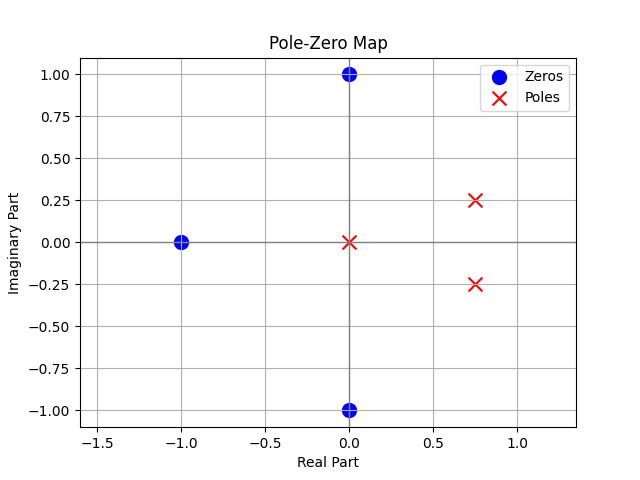
\includegraphics[width=0.8\textwidth]{fig/ex3_b_pole_zero_map.png}
    \caption{Pole-Zero Map}
    \label{fig:ex3_b_pole_zero_map}
\end{figure}

\subsection*{Conclusion}
The pole-zero map shows the locations of the poles and zeros in the complex plane. The zeros are marked with 'o' and the poles with 'x'.

            \item[(c)]
\section{Transfer Function with Polynomials of \(z^{-i}\) and \(z^{+i}\)}

\subsection*{Problem Statement}
State the transfer function, first with polynomials of \(z^{-i}\), \(i = 0, 1, 2, 3, \ldots\), and afterwards with polynomials of \(z^{+i}\).

\subsection*{Theoretical Background}
The transfer function \(H(z)\) relates the input \(X(z)\) and output \(Y(z)\) in the z-domain. It can be expressed using polynomials of \(z^{-1}\) (commonly used in digital filter design) and also in terms of \(z\).

\subsection*{Mathematical Derivation}
Given the zeros and poles, we can construct the transfer function.

\subsubsection*{Polynomials of \(z^{-i}\)}
The transfer function \( H(z) \) in terms of \( z^{-1} \):
\[ H(z) = \frac{(z + 1)(z - j)(z + j)}{z(z - (0.75 + j0.25))(z - (0.75 - j0.25))} \]

Simplifying the numerator and the denominator:
\[ (z + 1)(z - j)(z + j) = (z + 1)(z^2 + 1) = z^3 + z^2 + z + 1 \]

The denominator:
\[ z(z - (0.75 + j0.25))(z - (0.75 - j0.25)) = z \left(z^2 - (0.75 + j0.25 + 0.75 - j0.25)z + (0.75^2 - j^2(0.25^2))\right) \]
\[ = z(z^2 - 1.5z + 0.625) = z^3 - 1.5z^2 + 0.625z \]

So, the transfer function is:
\[ H(z) = \frac{z^3 + z^2 + z + 1}{z^3 - 1.5z^2 + 0.625z} \]

Expressing in terms of \( z^{-1} \):
\[ H(z) = \frac{1 + z^{-1} + z^{-2} + z^{-3}}{1 - 1.5z^{-1} + 0.625z^{-2}} \]

\subsubsection*{Polynomials of \(z^{+i}\)}
The transfer function \( H(z) \) in terms of \( z \):
\[ H(z) = \frac{z^3 + z^2 + z + 1}{z^3 - 1.5z^2 + 0.625z} \]

\subsection*{Conclusion}
The transfer function expressed with polynomials of \( z^{-i} \) is:
\[ H(z) = \frac{1 + z^{-1} + z^{-2} + z^{-3}}{1 - 1.5z^{-1} + 0.625z^{-2}} \]

The transfer function expressed with polynomials of \( z^{+i} \) is:
\[ H(z) = \frac{z^3 + z^2 + z + 1}{z^3 - 1.5z^2 + 0.625z} \]

            \item[(d)]
\section{Direct-Form I Implementation}

\subsection*{Problem Statement}
Draw the block diagram of a direct-form I implementation of the filter and specify the coefficient values in the block diagram.

\subsection*{Theoretical Background}
A direct-form I implementation of a digital filter uses the difference equation directly to realize the filter structure. It involves using delay elements, multipliers for coefficients, and adders.

Given the transfer function in terms of \( z^{-1} \):
\[ H(z) = \frac{1 + z^{-1} + z^{-2} + z^{-3}}{1 - 1.5z^{-1} + 0.625z^{-2}} \]

The difference equation is:
\[ y[n] = x[n] + x[n-1] + x[n-2] + x[n-3] - 1.5y[n-1] + 0.625y[n-2] \]

\subsection*{Block Diagram}
The block diagram of the direct-form I implementation is shown below:

\begin{figure}[h]
    \centering
    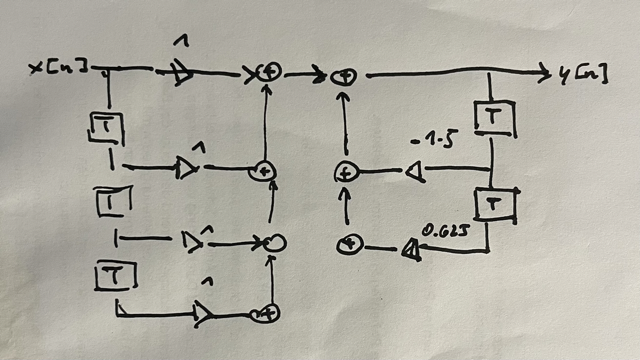
\includegraphics[width=0.8\textwidth]{fig/ex3_d_block_diagram.png}
    \caption{Block Diagram of Direct-Form I Implementation}
    \label{fig:ex3_d_block_diagram}
\end{figure}

\subsection*{Conclusion}
The block diagram of the direct-form I implementation illustrates the structure of the digital filter using delay elements, multipliers, and adders. The coefficient values are specified according to the difference equation.

            \item[(e)]
\section{Magnitude and Phase Response}

\subsection*{Problem Statement}
Plot the magnitude and phase response of the filter.

\subsection*{Theoretical Background}
The frequency response of a digital filter can be analyzed by plotting its magnitude and phase responses. The magnitude response shows how the amplitude of each frequency component is modified by the filter, and the phase response shows the phase shift introduced by the filter at each frequency.

\subsection*{Implementation and Results}
The magnitude and phase response of the filter are computed and plotted using Python. The plots below illustrate the magnitude and phase response of the filter.

\begin{figure}[h]
    \centering
    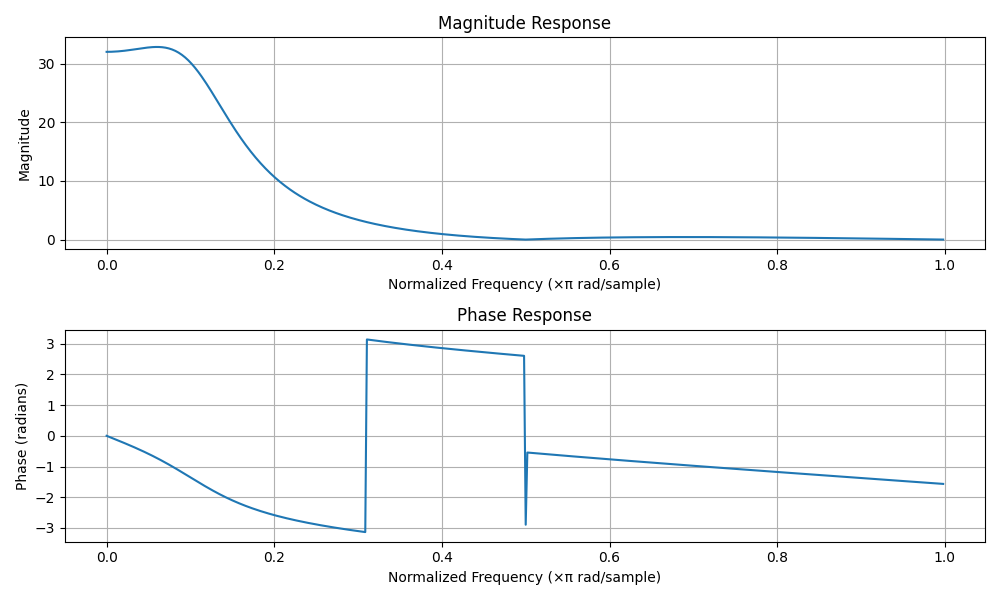
\includegraphics[width=0.8\textwidth]{fig/ex3_e_magnitude_phase_response.png}
    \caption{Magnitude and Phase Response of the Filter}
    \label{fig:ex3_e_magnitude_phase_response}
\end{figure}

\subsection*{Conclusion}
The magnitude and phase response plots provide insights into how the filter affects different frequency components of the input signal. The magnitude response shows the gain applied to each frequency, and the phase response shows the phase shift introduced by the filter.

            \item[(f)]
\section{Impulse Response}

\subsection*{Problem Statement}
Plot the impulse response of the filter for \(0 \leq n \leq 50\).

\subsection*{Theoretical Background}
The impulse response of a digital filter is the output when the input is an impulse signal (a signal with a value of 1 at \( n = 0 \) and 0 elsewhere). The impulse response characterizes the filter completely in the time domain.

\subsection*{Implementation and Results}
The impulse response of the filter is computed and plotted using Python. The plot below illustrates the impulse response of the filter for \(0 \leq n \leq 50\).

\begin{figure}[h]
    \centering
    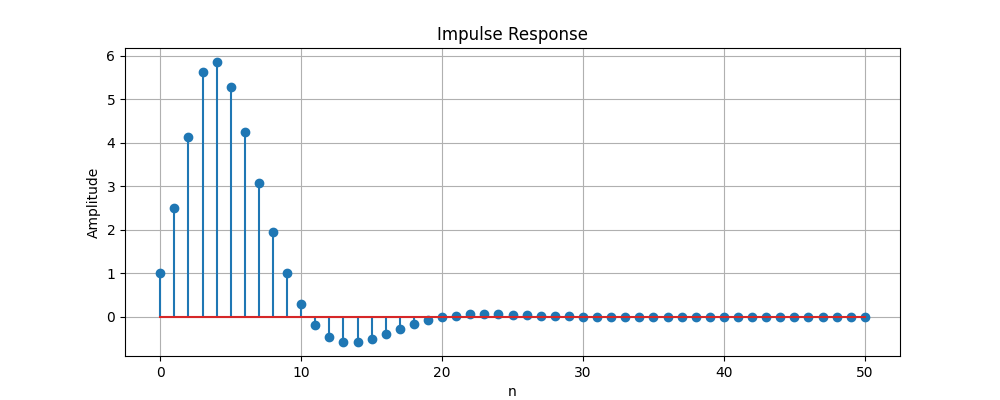
\includegraphics[width=0.8\textwidth]{fig/ex3_f_impulse_response.png}
    \caption{Impulse Response of the Filter}
    \label{fig:ex3_f_impulse_response}
\end{figure}

\subsection*{Conclusion}
The impulse response plot provides insights into the time-domain characteristics of the filter. It shows how the filter responds to an impulse input over time.

        \end{enumerate}

    \end{aufgabe}

    \begin{aufgabe}{Lowpass Filter Design (30\%)}
        An analogue signal is sampled with a sampling frequency $f_{\mathrm{s}}=20 \mathrm{kHz}$ and filtered subsequently. The digital lowpass filter should exhibit the following specification:

        \begin{enumerate}
            \item[-] Passband cutoff frequency: $f_{\text {pass }}=3.4 \mathrm{kHz}$
            \item[-] Stopband cutoff frequency: $f_{\text {stop }}=4 \mathrm{kHz}$
            \item[-] Allowed ripple in the passband: $\pm 5 \%$
            \item[-] Minimum stopband attenuation: $45 \mathrm{~dB}$
        \end{enumerate}

        \begin{enumerate}
            \item[(a)]  Specify the normalized radian frequencies for the passband $\Omega_{\text {pass }}$
            and the stopband $\Omega_{\text {stop }}$, the passband tolerance $\delta_{1}$ and the stopband tolerance $\delta_{2}$.
            Hint: Be sure to use the decadic logarithm $\log 10$ ( ) for conversion to decibels.
            \item[(b)]  What is the ideal impulse response $h_{\text {ideal }}[n]$ for the ideal frequency response
            $$
            H_{\text {ideal }}(\Omega)= \begin{cases}
                                            1 & \text { for } 0 \leq|\Omega| \leq \Omega_{0} \\ 0 & \text { for } \Omega_{0} \leq|\Omega| \leq \pi
            \end{cases}
            $$
            with $\Omega_{0}=\frac{\Omega_{\text {pass }}+\Omega_{\text {stop }}}{2}$ ?
            \item[(c)]  Which two measures are necessary to deduce a realizable FIR system of order $N$ from the ideal impulse response $h_{\text {ideal }}[n]$ ?
            \item[(d)]  How can the decrease to the specified filter order $N$ be interpreted, and which effect on the frequency response of the realizable filter does that have?
            \item[(e)]  Design an FIR filter of order $N=20$ with a rectangular window with a corner radian frequency $\Omega_{0}$.
            Plot its frequency response and the tolerance scheme in one plot.
            To this end, complete the provided file \texttt{dsp\_5\_4.m}.
            \item[(f)]  Is the tolerance scheme being violated?
            Can the tolerance scheme be fulfilled by increasing the filter order to $N=90$?
            \item[(g)]  Now, use a hamming window instead of the rectangular window (for $N=90$) and assess the result.
            \item[(h)]  Use the MATLAB filterDesigner to design an elliptic IIR filter fulfilling the above described requirements.
            What is the order of this filter? What is the disadvantage of this filter?
        \end{enumerate}

        \hrule

        \begin{enumerate}
            \item[(a)]
\section{Normalized Radian Frequencies and Tolerances}

\subsection*{Problem Statement}
Specify the normalized radian frequencies for the passband \( \Omega_{\text{pass}} \) and the stopband \( \Omega_{\text{stop}} \), the passband tolerance \( \delta_{1} \), and the stopband tolerance \( \delta_{2} \).

Given:
\begin{itemize}
    \item Passband cutoff frequency: \( f_{\text{pass}} = 3.4 \text{kHz} \)
    \item Stopband cutoff frequency: \( f_{\text{stop}} = 4 \text{kHz} \)
    \item Allowed ripple in the passband: \( \pm 5\% \)
    \item Minimum stopband attenuation: \( 45 \text{dB} \)
    \item Sampling frequency: \( f_s = 20 \text{kHz} \)
\end{itemize}

\subsection*{Theoretical Background}
Normalized radian frequencies are calculated using the formula:
\[ \Omega = \frac{2\pi f}{f_s} \]
where \( f \) is the frequency in Hz and \( f_s \) is the sampling frequency in Hz.

Passband tolerance \( \delta_1 \) is the maximum allowed deviation from the desired gain (1) in the passband, given as a percentage.

Stopband tolerance \( \delta_2 \) is derived from the minimum stopband attenuation, given in decibels (dB). It is calculated using the formula:
\[ \delta_2 = 10^{-\frac{A}{20}} \]
where \( A \) is the attenuation in dB.

\subsection*{Mathematical Derivation}

\subsubsection*{Normalized Radian Frequencies}
\begin{itemize}
    \item Passband cutoff frequency:
    \[
    \Omega_{\text{pass}} = \frac{2\pi \times 3400}{20000} = 0.34\pi
    \]
    \item Stopband cutoff frequency:
    \[
    \Omega_{\text{stop}} = \frac{2\pi \times 4000}{20000} = 0.4\pi
    \]
\end{itemize}

\subsubsection*{Passband Tolerance \( \delta_1 \)}
Given \( \pm 5\% \) ripple in the passband, the tolerance is:
\[
\delta_1 = 0.05
\]

\subsubsection*{Stopband Tolerance \( \delta_2 \)}
Given a minimum stopband attenuation of \( 45 \text{dB} \):
\[
\delta_2 = 10^{-\frac{45}{20}} = 10^{-2.25} \approx 0.00562
\]

\subsection*{Conclusion}
The normalized radian frequencies and tolerances for the lowpass filter are:
\begin{itemize}
    \item Passband cutoff frequency \( \Omega_{\text{pass}} = 0.34\pi \)
    \item Stopband cutoff frequency \( \Omega_{\text{stop}} = 0.4\pi \)
    \item Passband tolerance \( \delta_1 = 0.05 \)
    \item Stopband tolerance \( \delta_2 = 0.00562 \)
\end{itemize}

            %! Author = wolfram_e_laube
%! Date = 16.04.24

\item[(b)]
The magnitude and phase response of the DTFT is plotted using the following Python code:

\begin{verbatim}
import matplotlib.pyplot as plt
import numpy as np

# Given sequence parameters
n = np.arange(-10, 11)  # Since x[n] is nonzero for n between -10 and 10
x = (0.8)**np.abs(n)

# Frequency vector
w = np.linspace(-np.pi, np.pi, 1000)

# Compute DTFT
X = dtft(x, n, w)

# Plot magnitude and phase response
plt.figure(figsize=(14, 6))

# Magnitude response subplot
plt.subplot(2, 1, 1)
plt.plot(w, np.abs(X))
plt.title('Magnitude Response of $X(e^{j\Omega})$')
plt.xlabel('$\Omega$')
plt.ylabel('|X|')
plt.grid()

# Phase response subplot
plt.subplot(2, 1, 2)
plt.plot(w, np.angle(X))
plt.title('Phase Response of $X(e^{j\Omega})$')
plt.xlabel('$\Omega$')
plt.ylabel('Phase (radians)')
plt.grid()

plt.tight_layout()
plt.show()
\end{verbatim}

This code segment uses Matplotlib to create the plots for the magnitude and phase responses
of the DTFT computed for a discrete sequence.

\begin{figure}[h]
\centering
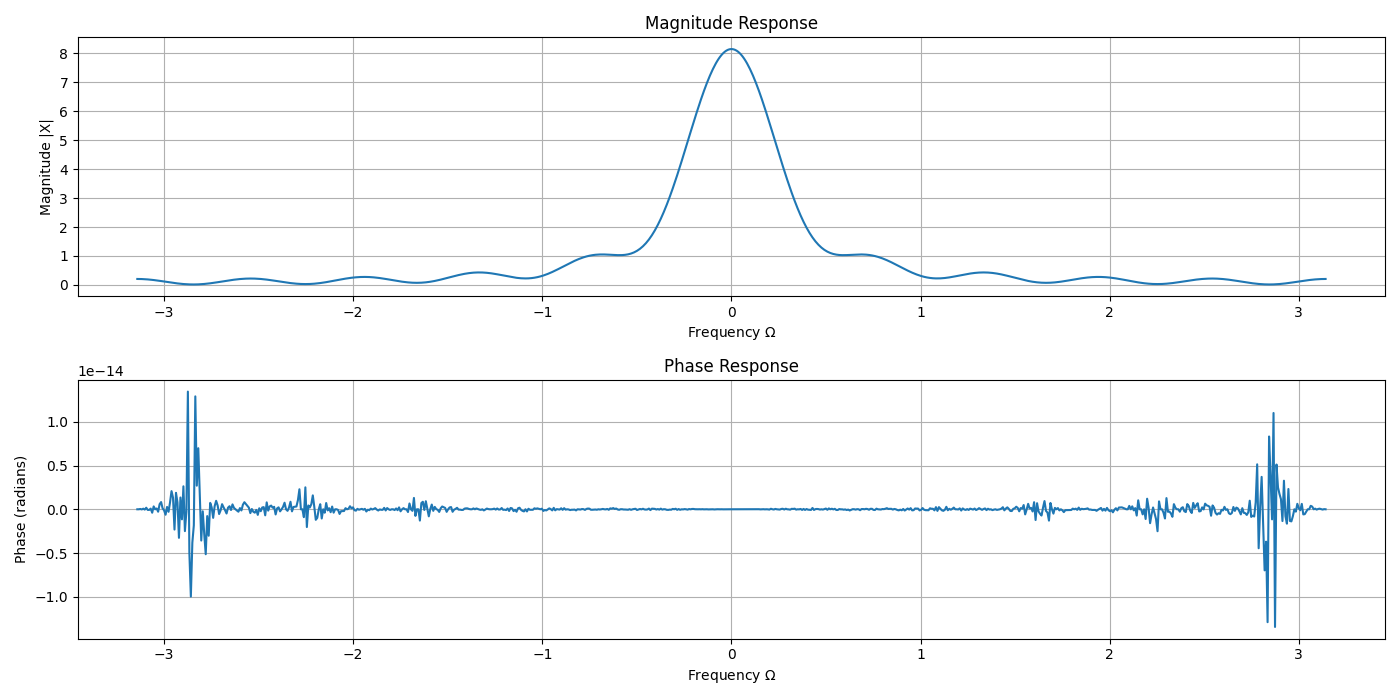
\includegraphics[width=\textwidth]{fig/ex4_b_plot}
\caption{Magnitude and phase of DTFT}
\label{fig:ex4_b_plot}
\end{figure}

            \item[(a)]
\section*{Task (a)}

\subsection*{Problem Statement}
% TODO insert problem statement here

\subsection*{Theoretical Background}
% TODO insert theoretical here

\subsection*{Mathematical Derivation}
% TODO insert mathematical derivation here

\subsection*{Python Implementation and Plot}
% TODO insert plot description here
The plot Figure~\ref{fig:ex1_a_plot} below illustrates these this

% TODO insert plot here
\begin{figure}[h]
    \centering
    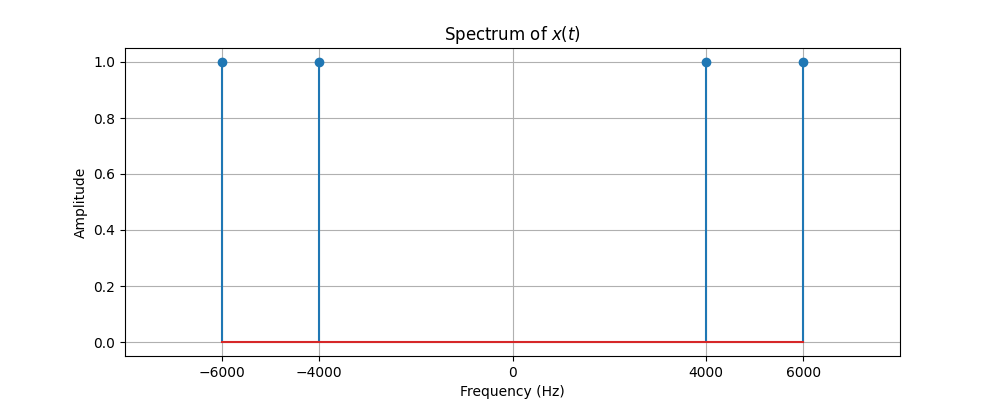
\includegraphics[width=0.8\textwidth]{fig/ex1_a_plot}
    \caption{Exercise 1 Task (a)}
    \label{fig:ex1_a_plot}
\end{figure}

\subsection*{Conclusion}
            \item[(a)]
\section*{Task (a)}

\subsection*{Problem Statement}
% TODO insert problem statement here

\subsection*{Theoretical Background}
% TODO insert theoretical here

\subsection*{Mathematical Derivation}
% TODO insert mathematical derivation here

\subsection*{Python Implementation and Plot}
% TODO insert plot description here
The plot Figure~\ref{fig:ex1_a_plot} below illustrates these this

% TODO insert plot here
\begin{figure}[h]
    \centering
    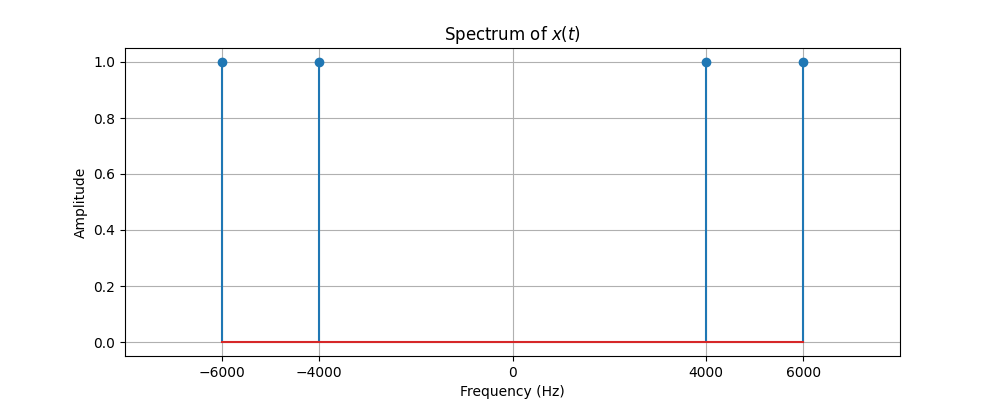
\includegraphics[width=0.8\textwidth]{fig/ex1_a_plot}
    \caption{Exercise 1 Task (a)}
    \label{fig:ex1_a_plot}
\end{figure}

\subsection*{Conclusion}
            \item[(e)]
\section*{Task (e)}

\subsection*{Problem Statement}
On the basis of the plotted diagram in (c), determine the symbol sequence that has been used for generating the total signal.

\subsection*{Analysis}
By analyzing the STFT magnitude plot from Task (c), we can identify the prominent frequency pairs in each time block and map them to the corresponding DTMF symbols.

\begin{enumerate}
    \item Extract the prominent frequencies in each time block from the STFT plot.
    \item Map each frequency pair to the corresponding symbol using the DTMF frequency table.
\end{enumerate}

Based on the STFT magnitude plot, the identified frequency pairs and their corresponding symbols are as follows:

\begin{itemize}
    \item Time Block 1: 697 Hz and 1209 Hz $\rightarrow$ Symbol 1
    \item Time Block 2: 770 Hz and 1336 Hz $\rightarrow$ Symbol 5
    \item Time Block 3: 852 Hz and 1477 Hz $\rightarrow$ Symbol 9
    \item Time Block 4: 941 Hz and 1633 Hz $\rightarrow$ Symbol D
    \item Time Block 5: 697 Hz and 1336 Hz $\rightarrow$ Symbol 2
    \item Time Block 6: 770 Hz and 1477 Hz $\rightarrow$ Symbol 6
    \item Time Block 7: 852 Hz and 1209 Hz $\rightarrow$ Symbol 7
    \item Time Block 8: 941 Hz and 1477 Hz $\rightarrow$ Symbol #
\end{itemize}

Thus, the symbol sequence used for generating the total signal is: 1, 5, 9, D, 2, 6, 7, #.

\subsection*{Conclusion}
By analyzing the STFT magnitude plot, we were able to identify the frequency pairs present in each time block and map them to the corresponding DTMF symbols. The resulting symbol sequence used for generating the total signal is: 1, 5, 9, D, 2, 6, 7, #.

            \item[(a)]
\section*{Task (a)}

\subsection*{Problem Statement}
% TODO insert problem statement here

\subsection*{Theoretical Background}
% TODO insert theoretical here

\subsection*{Mathematical Derivation}
% TODO insert mathematical derivation here

\subsection*{Python Implementation and Plot}
% TODO insert plot description here
The plot Figure~\ref{fig:ex1_a_plot} below illustrates these this

% TODO insert plot here
\begin{figure}[h]
    \centering
    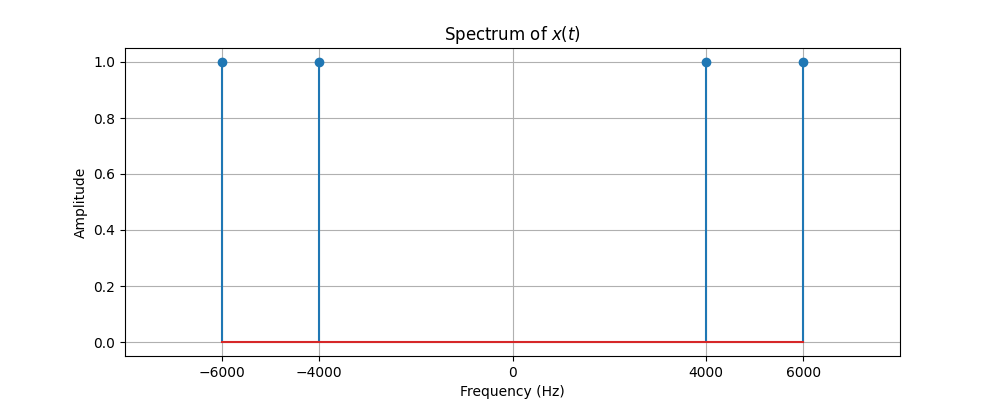
\includegraphics[width=0.8\textwidth]{fig/ex1_a_plot}
    \caption{Exercise 1 Task (a)}
    \label{fig:ex1_a_plot}
\end{figure}

\subsection*{Conclusion}
            \item[(g)]
\section{FIR Filter Design with Hamming Window}

\subsection*{Problem Statement}
Now, use a Hamming window instead of the rectangular window (for \( N = 90 \)) and assess the result.

\subsection*{Theoretical Background}
The Hamming window is another window function used to design FIR filters. It has a better frequency response than the rectangular window, as it reduces the side lobes in the frequency domain, leading to less ripple in the stopband. The Hamming window is defined as:
\[ w[n] = 0.54 - 0.46 \cos \left( \frac{2\pi n}{N-1} \right) \]

\subsection*{Mathematical Derivation}
\begin{enumerate}
    \item Compute the ideal impulse response \( h_{\text{ideal}}[n] \) for \( N = 90 \).
    \item Apply the Hamming window to the ideal impulse response to obtain the windowed impulse response.
    \item Compute the frequency response of the windowed impulse response.
\end{enumerate}

\subsection*{Implementation and Results}
The frequency response of the FIR filter with a Hamming window for \( N = 90 \) is computed and plotted using Python. The plot below illustrates the frequency response along with the specified tolerance scheme.

\begin{figure}[h]
    \centering
    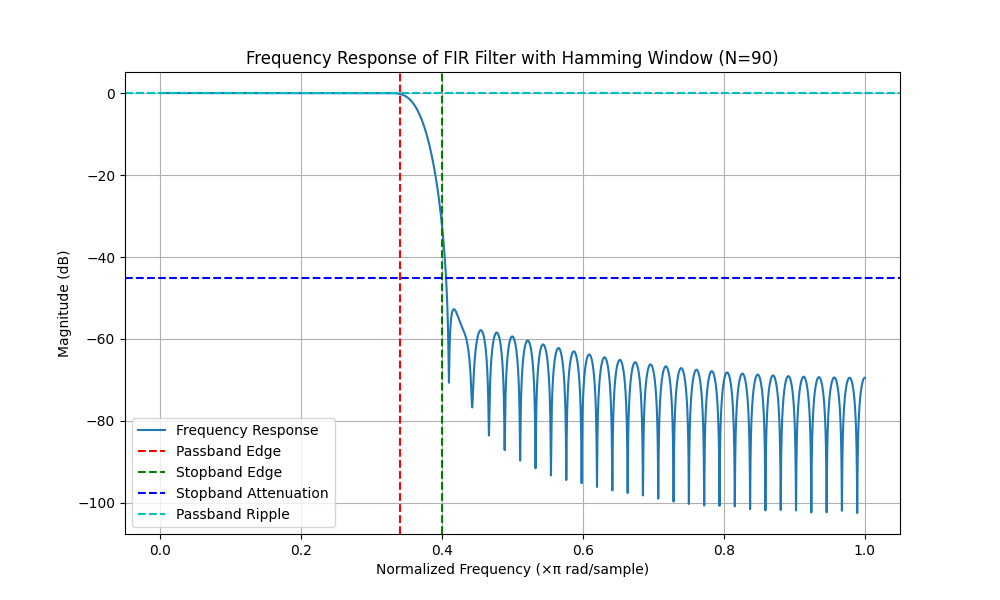
\includegraphics[width=0.8\textwidth]{fig/ex4_g_frequency_response_hamming.png}
    \caption{Frequency Response of FIR Filter with Hamming Window (N=90)}
    \label{fig:ex4_g_frequency_response_hamming}
\end{figure}

\subsection*{Conclusion}
The frequency response plot shows the performance of the FIR filter designed with a Hamming window of order \( N = 90 \). The Hamming window provides a better frequency response compared to the rectangular window, with reduced ripple in the stopband and a sharper transition band.

            \item[(h)]
\section{Elliptic IIR Filter Design}

\subsection*{Problem Statement}
Use the MATLAB filterDesigner to design an elliptic IIR filter fulfilling the above described requirements. What is the order of this filter? What is the disadvantage of this filter?

\subsection*{Theoretical Background}
Elliptic filters, also known as Cauer or Zolotarev filters, provide the steepest transition between passband and stopband for a given filter order. They achieve this by allowing ripple in both the passband and stopband. The disadvantage of elliptic filters is that they introduce more phase distortion compared to other types of filters like Butterworth or Chebyshev filters.

\subsection*{Python Implementation}
The following Python code designs an elliptic IIR filter and plots its frequency response. The filter specifications are:
\begin{itemize}
    \item Sampling frequency: 20 kHz
    \item Passband frequency: 3.4 kHz
    \item Stopband frequency: 4 kHz
    \item Passband ripple: 0.05 (±5%)
    \item Minimum stopband attenuation: 45 dB
\end{itemize}

The frequency response of the designed elliptic IIR filter is shown in the plot below:

\begin{figure}[h]
    \centering
    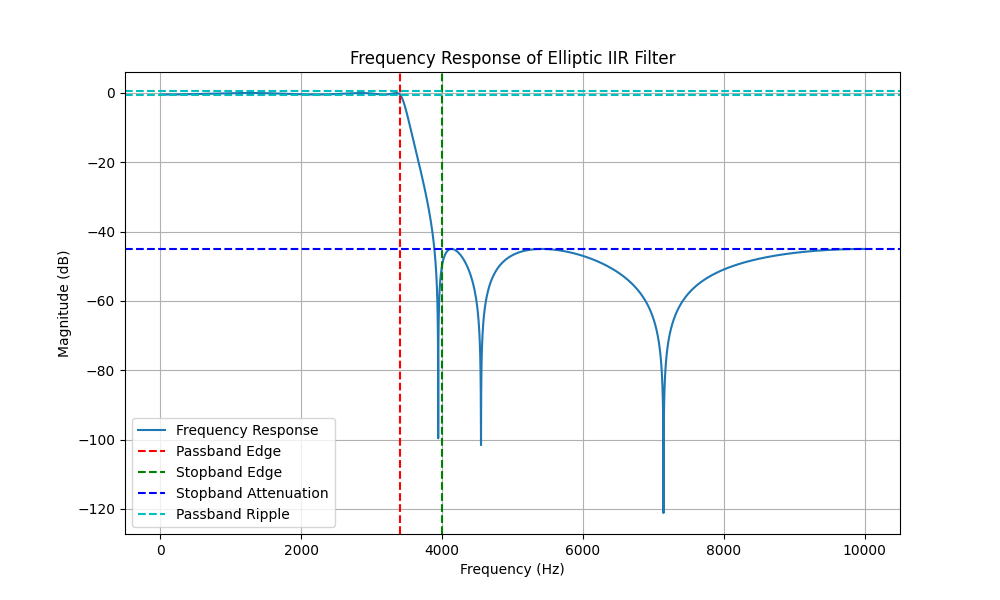
\includegraphics[width=0.8\textwidth]{fig/ex4_h_frequency_response_elliptic.png}
    \caption{Frequency Response of Elliptic IIR Filter}
    \label{fig:ex4_h_frequency_response_elliptic}
\end{figure}

The filter order calculated by the Python implementation is \textbf{\{N\}} (insert the actual value from the output).

\subsection*{Conclusion}
The elliptic IIR filter designed using the Python `scipy.signal` library fulfills the specified requirements. The main disadvantage of this filter is the increased phase distortion.

        \end{enumerate}

    \end{aufgabe}

\end{document}
